\documentclass[10pt]{article}

\usepackage{amsfonts, amsthm, amsmath, enumerate, tikz, fullpage}

\newcommand{\card}[1]{\left| #1 \right|}
\newcommand{\brackets}[1]{\left< #1 \right>}
\newcommand{\nat}{\mathbb{N}}
\newcommand{\ints}{\mathbb{Z}}
\newcommand{\reals}{\mathbb{R}}
\newcommand{\chtitle}[1]{\noindent \vspace{5mm}\textbf{Chapter #1}\vspace{3mm}}

\begin{document}
\begin{flushleft}
\textbf{\noindent
STUDENT NAME - EID\\
CS 341 Automata Theory \\
Homework 16 \\
Due Friday, May 4 at 11:59 p.m.}\\
\end{flushleft}

\noindent
This assignment reviews Chapter 21 and covers Chapter 27 and part of Chapter 28.\\

\begin{enumerate}[1)]

% ---
% 1
% ---

\item
For each of the following languages $L$, state whether it is in D, SD/D or not SD.  Prove your answer.  Do not use
Rice’s Theorem.  If you claim that $L$ is not in SD, first prove that it’s not in D (for practice), then prove that it’s not
in SD.  Assume that any input of the form $\brackets{M}$ is a description of a Turing machine.
\begin{enumerate}[a)]
\item
\{$\brackets{M}$ : $L(M)$ contains at least two strings\}.
\begin{proof}[Answer]
\end{proof}
\begin{proof}[Proof]
\end{proof}
\item
\{$\brackets{M}$ : $M$ is the only Turing machine that accepts $L(M)$\}.
\begin{proof}[Answer]
\end{proof}
\begin{proof}[Proof]
\end{proof}
\item
\{$\brackets{M}$ : $\card{L(M)}$ is a prime integer $> 0$\}.
\begin{proof}[Answer]
\end{proof}
\begin{proof}[Proof]
\end{proof}
\end{enumerate}

%---
% 2
%---

\item
Let $Oops$ be a function-computing TM defined as follows:
\begin{center}
\begin{tabular}{p{2cm} l}
Input:&$\brackets{id, c}$, where $id$ is a student id for student $s$ and $c$ is a course number.\\
Output:&The grade to be assigned to student $s$ in course $c$.
\end{tabular}
\end{center}

For whatever reason (malevolence or incompetence), it turns out that $Oops$ has the property that, for all input pairs, it outputs the value \texttt{F}.\\

For this problem, we’ll say that two TMs are equivalent iff they compute the same function (i.e., they halt on the same inputs and, when they halt, they output the same value).\\

Define $L = \{\brackets{M}$ : $M$ is equivalent to $Oops$\}.  Is $L$ in D, SD/D or $\lnot$SD?  Prove your answer.
\begin{proof}[Answer]
\end{proof}
\begin{proof}[Proof]
\end{proof}

% ---
% 3
% ---

\item
Let $M$ be an arbitrary Turing machine.
\begin{enumerate}[a)]
\item
Suppose that $timereq(M) = 3n^3(n+5)(n-4)$.  Circle all of the following statements that are true:
\begin{enumerate}[i]
\item
$timereq(M) \in O(n)$.
\item
$timereq(M) \in O(n^6)$.
\item
$timereq(M) \in O(\frac{n^5}{50})$.
\item
* $timereq(M) \in \Theta(n^6)$.
\end{enumerate}
\begin{proof}[Answer]
\end{proof}

\item
Suppose that $timereq(M) = 5^n \cdot 3n^3$.  Circle all of the following statements that are true:
\begin{enumerate}[i)]
\item
$timereq(M) \in O(n^5)$.
\item
$timereq(M) \in O(2^n)$.
\item
$timereq(M) \in O(n!)$.
\end{enumerate}
\begin{proof}[Answer]
\end{proof}
\end{enumerate}

% ---
% 4
% ---

\item
* Let $M$ be the Turing machine shown in Example 17.9.  $M$ accepts the language\\ W\texttt{c}W $= \{w\texttt{c}w\ :\ w \in \{a, b\}^*\}$.
\begin{enumerate}[a)]
\item
Analyze $timereq(M)$.
\begin{proof}[Answer]
\end{proof}
\item
Is W\texttt{c}W in P?  Why (or why do you think it’s not)?
\begin{proof}[Answer]
\end{proof}
\end{enumerate}

% ---
% 5
% ---

\item
Assume a computer that executes $10^{10}$ operations/second.  Make the simplifying assumption that each operation of a program requires exactly one machine instruction.  For each of the following programs $P$, defined by its time requirement, what is the largest size input on which $P$ would be guaranteed to halt within a week?
\begin{enumerate}[a)]
\item
$timereq(P) = 5243n+649$.
\begin{proof}[Answer]
\end{proof}
\item
* $timereq(P) = 5n^2$.
\begin{proof}[Answer]
\end{proof}
\item
* $timereq(P) = 5^n$.
\begin{proof}[Answer]
\end{proof}
\end{enumerate}


% ---
% 6
% ---

\item
* Let each line of the following table correspond to a problem for which two algorithms, $A$ and $B$, exist.  The table entries correspond to $timereq$ for each of those algorithms.  Determine, for each problem, the smallest value of $n$ (the length of the input) such that algorithm $B$ runs faster than algorithm $A$.
\begin{center}
\begin{tabular}{| p{3cm} | p{3cm} |}
  \hline
  \multicolumn{1}{|c}{A}&
  \multicolumn{1}{|c|}{B}\\
  \hline
  $n^2$&$572n + 4171$\\
  \hline
  $n^2$&$1000n\textrm{ log}_2\ n$\\
  \hline
  $n!$&$450n^2$\\
  \hline
  $n!$&$3^n + 2$\\
  \hline
\end{tabular}
\end{center}
\begin{proof}[Answer]
\end{proof}

% ---
% 7
% ---

\item
Show that $L = \{\brackets{M}:\ M$ is a Turing machine and $timereq(M) \in O(n^2)\}$ is not in SD.
\begin{proof}[Proof]
\end{proof}

% ---
% 8
% ---

\item
In Section 28.1.5, we described the Seven Bridges of Königsberg.  Consider the following modification:\\

\begin{center}
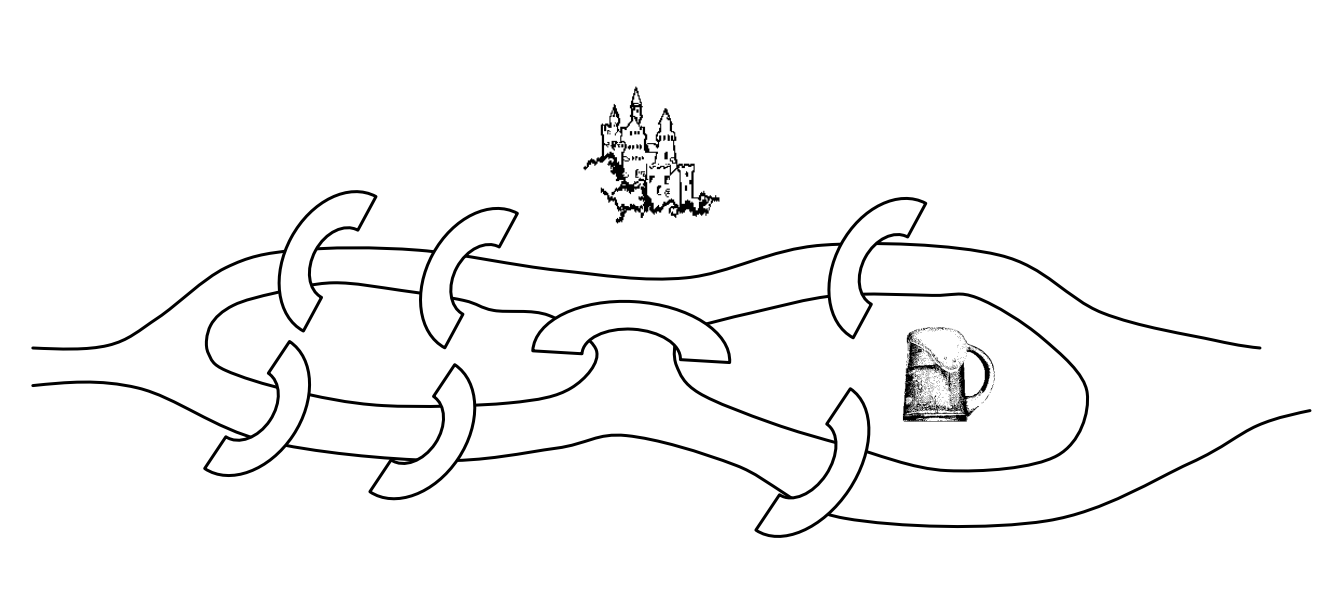
\includegraphics[scale=.25]{images/bridges.png}
\end{center}

The good prince lives in the castle.  He wants to be able to return home from the pub (on one of the islands as
shown above) and cross every bridge exactly once along the way.  But he wants to make sure that his evil twin,
who lives on the other river bank, is unable to cross every bridge exactly once on his way home from the pub.  The
good prince is willing to invest in building one new bridge in order to make his goal achievable.  Where should he
build his bridge?
\begin{proof}[Answer]
\end{proof}

% ---
% 9
% ---

\item
* Consider the language NONEULERIAN $= \{\brackets{G}$ : $G$ is an undirected graph and $G$ does not contain an Eulerian
circuit\}.
\begin{enumerate}[a)]
\item
Show an example of a connected graph with 8 vertices that is in NONEULERIAN.
\begin{proof}[Answer]
\end{proof}
\item
Prove that NONEULERIAN is in P.
\begin{proof}[Proof]
\end{proof}
\end{enumerate}

% ---
% 10
% ---

\item
In Chapter 9, we showed that all of the questions that we posed about regular languages are decidable.  It is shown,
in Section 29.3.3, that while decidable, some straightforward questions about the regular languages appear to be
hard.  Some are easy however.  Show that FSM-EMPTY = \{$\brackets{M}$ : $M$ is a FSM and $L(M) = \emptyset$\} is in P.
\begin{proof}[Proof]
\end{proof}

% ---
% 11
% ---

\item
* Show that SUBSET-SUM = \{$\brackets{S, k}$ : $S$ is a multiset (i.e., duplicates are allowed) of integers, $k$ is an integer, and
there exists some subset of $S$ whose elements sum to $k$\} is in NP.
\begin{proof}[Proof]
\end{proof}

% ---
% 12
% ---

\item
* In Section 22.3, we introduced a family of tiling problems and defined the language TILES.  In that discussion, we considered the question, “Given an infinite set $T$ of tile designs and an infinite number of copies of each such design, is it possible to tile every finite surface in the plane?”  As we saw there, that unbounded version of the problem is undecidable.  Now suppose that we are again given a set $T$ of tile designs.  But, this time, we are also given $n^2$ specific tiles drawn from that set.  The question we now wish to answer is, “Given a particular stack of $n^2$ tiles, is it possible to tile an $n \times n$ surface in the plane?”  As before, the rules are that tiles may not be rotated or flipped and the abutting regions of every pair of adjacent tiles must be the same color.  So, for example, suppose that the tile set is:\\
\begin{center}

\includegraphics[scale=.5]{images/tileset.jpg}
\end{center}
Then a $2 \times 2$ grid can be tiled as:\\
\begin{center}
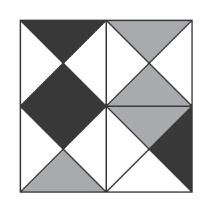
\includegraphics[scale=.5]{images/tiling.jpg}
\end{center}
\begin{enumerate}[a)]
\item
Formulate this problem as a language, FINITE-TILES
\begin{proof}[Solution]
\end{proof}
\item
Show that FINITE-TILES is in NP.
\begin{proof}[Proof]
\end{proof}
\end{enumerate}
\end{enumerate}
\end{document}
